\chapter{Análisis del sistema}

%Todo el análisis previo al diseño y desarrollo del sistema, hasta cierto punto lo más de hueva que se tienen que hacer pero que fundamenta el porque realizar el trabajo. Las secciones que deberiamos cubrir en este apartado son las siguientes:
%
%\begin{itemize}
%    \item Factibilidad
%        \begin{itemize}
%            \item técnica
%            \item operativa
%            \item económica
%            \item analisis de factibilidad (conclusiones con base en los tres puntos anteriores)
%        \end{itemize}
%    \item Requerimientos
%        \begin{itemize}
%            \item funcionales
%            \item no funcionales
%            \item operativos o de sistema
%        \end{itemize}
%    \item Reglas de negocio
%    \item Análisis de riesgos
%    \item Descripción del software
%    \item Herramientas de desarrollo
%    \item Metodología
%\end{itemize}

\section{Requerimientos funcionales}
    Los requerimientos funcionales describen los actividades y comportamientos que tendrá el sistema bajo ciertas condiciones, de igual forma pueden declarar lo que el sistema no debe de hacer.
    
    En esta sección se presentan los requerimientos funcionales que se obtuvieron para el sistema. Dichos requerimientos se encuentran separados de acuerdo a los diferentes módulos que se tienen planeados.
    \subsection{Módulo de usuarios}
    \begin{enumerate}[label=\textbf{RF\arabic*.}]
    \item \textbf{Mecanismo de gestión de usuarios.} Proporcionar al usuario la posibilidad de creación, consulta y modificación de los datos de su cuenta de usuario. Estas operaciones debe de estar presentes en la aplicación web y de android y solo serán permitidas para usuarios con cuenta verificada.
    \item \textbf{Mecanismo de autenticación de usuarios.} Proporcionar un mecanismo para el inicio y cierre de sesión de la cuenta del usuario cuya cuenta haya sido verificada en la aplicación web y android.
    \item \textbf{Mecanismo de verificación de cuenta.} Proporcionar al usuario una forma para verificar que una cuenta creada es valida a través de una verificación basada en el envió de un correo electrónico para la confirmar dicha validez y hacer uso del resto de funcionalidad del sistema. Esta verificación solo se podra realizar a través de la aplicación web.
    \item \textbf{Mecanismo de recuperación de contraseñas.} Proporcionar al usuario la posibilidad de recuperar la contraseña asociada a su cuenta a través de un envío de correo electrónico con el cual podrá acceder a una interfaz en la aplicación web para recuperar el acceso a su cuenta. La recuperación de contraseñas estará disponible en la aplicación android y web.
    \item \textbf{Mecanismo para la comunicación entre la aplicación android y web.} El sistema debe de contar con una interfaz para la comunicación entre las dos aplicaciones que se tienen, la forma en que se realizara sera un API REST y el formato para el envió de información sera JSON.
    \item \textbf{Mecanismo para la autenticación en el API REST.} El sistema debe de brindar una forma de garantizar que la comunicación entre la aplicación web y android es seguro mediante el uso de tokens de autenticación en cada petición y respuesta que se realice.
    \end{enumerate}
    
    \subsection{Módulo de proyectos}
    \begin{enumerate}[label=\textbf{RF\arabic*.}]
    	\setcounter{enumi}{4}
    	\item \textbf{Mecanismo para la gestión de proyectos de \LaTeX{}.} Proporcionar al usuario un mecanismo para visualizar, editar, crear o borrar proyectos asociados a su cuenta. La gestión se podrá realizar en la aplicación web y android.
    	\item \textbf{Permitir descargar el archivo de \LaTeX{}} que se haya traducido. Proporcionar al usuario la funcionalidad de generar un archivo \LaTeX{} que contenga la traducción de expresiones matemáticas que se encuentren en un proyecto. La descarga de dicho archivo solo estará disponible en la aplicación web.
    	\item \textbf{Permitir calificar una traducción realizada.} Proporcionar al usuario la funcionalidad de calificar que tan buena fue la traducción de una expresión matemática en una imagen para brindar retroalimentación, dicha calificación podrán ser valores enteros entre 1 y 5. Para poder calificar una traducción se tendrá que hacer uso de la aplicación web.
    	\item \textbf{Permitir el uso de la cámara del dispositivo android para tomar fotografías.} Proporcionar un mecanismo en la aplicación web que permita acceder a la cámara del dispositivo, tomar una fotografía, visualizarla.
    	\item \textbf{Permitir la visualización del resultado de la traducción.} Proporcionar al usuario una interfaz en la cual pueda observar la traducción a \LaTeX{} que se realizó a partir de una imagen. Esto se podrá hacer en la aplicación web y android.
    	\item \textbf{Permitir añadir al portapapeles alguna traducción seleccionada.} Proporcionar al usuario la funcionalidad para copiar el código de una traducción a su portapapeles para su posterior uso. Esta funcionalidad está limitada a solo la aplicación web.
    	\item \textbf{Mecanismo para el envío de imágenes tomadas por la aplicación android a la aplicación web para su uso.} El sistema debe de tener un mecanismo que a través del uso del API REST permita a la aplicación android el enviar una imagen a la aplicación web para que esta sea tratada. 
    \end{enumerate}
    
    \subsection{Módulo de análisis}
    \begin{enumerate}[label=\textbf{RF\arabic*.}]
    	\setcounter{enumi}{11}
    	\item \textbf{Mecanismo para el tratamiento de la imagen previo a su análisis.} El sistema deberá de realizar un tratamiento al imagen que reciba de la aplicación android para hacer que esta sea más sencilla de trabajar destacando sus partes importantes.
    	\item \textbf{Mecanismo para el reconocimiento de un conjunto definido de expresiones matemáticas en imágenes.} El sistema deberá de reconocer ciertas expresiones en particular con la posibilidad de que expresiones que no se encuentren en este conjunto produzcan resultados no esperados.
    \end{enumerate}
    
    \subsection{Módulo de traducción}
    \begin{enumerate}[label=\textbf{RF\arabic*.}]
    	\setcounter{enumi}{13}
    	\item \textbf{Mecanismo para la traducción a \LaTeX{} de las expresiones matemáticas encontradas en el modulo de análisis.} Implementar un algoritmo basado de gramáticas, redes neuronales o arboles de recubrimiento mínimo que permita transformar la salida que proporcione el módulo de análisis a código \LaTeX que pueda ser interpretado por un compilador.
    \end{enumerate}
    
\section{Requerimientos No Funcionales} 
    A continuación se enlistan los requerimientos no funcionales.
        \begin{enumerate}[label=RNF\arabic*.]
            \item Usabilidad. La interfaz de usuario debe de ser intuitiva con el objetivo de hacer uso de las funcionalidades del sistema de una forma fácil para el usuario.
            
            \item Seguridad. La seguridad se solventa al realizar un cifrado de las contraseñas de los usuarios así como una verificación de la cuenta del usuario para poder hacer uso del sistema. Por otro lado, en la comunicación que se realiza entre la aplicación móvil y el API REST se utiliza un token para autenticar las peticiones que se realizan, dicho token es único para cada usuario. 
            
            \item Escalabilidad. El sistema deberá ser fácilmente escalable y con ello poseer la cualidad de que si se agregan nuevas funcionalidades, estas sean fáciles de acoplar con lo ya desarrollado. Además, de que debe de ser posible aumentar sus capacidades para brindar servicio a más usuarios.
            
            \item Disponibilidad. El sistema debería estar disponible en la mayor parte del tiempo, para lograr esto el uso de un proveedor de hosting es necesario. Entre las posibles opciones están Amazon Web Services, Azure o Google Cloud
            
        \end{enumerate}    
\section{Requerimientos técnicos}
    A continuación se en listan los requerimientos técnicos para un mejor funcionamiento del sistema:
    \subsection{Aplicación móvil}
    \subsubsection{Requerimientos mínimos de software}
    \begin{enumerate}
        \item Sistema operativo Android 4.5 o superior.
        \item Conexión a internet.
    \end{enumerate}
    
    \subsubsection{Requerimientos mínimos de hardware}
    \begin{enumerate}
        %\item Resolución cámara: 13 Megapixeles
        %\item Procesador: Dualcore de 1.2 GHz.
        \item Memoria RAM: 2 GB.
        \item Espacio de almacenamiento de 50 MB.
        \item Cámara de al menos 8 Megapixeles.
    \end{enumerate}
    \subsection{Aplicación web}
    \subsubsection{Requerimientos mínimos de software}
    \begin{enumerate}
        \item Cualquiera de las versiones de los siguientes navegadores hasta su versión más reciente.
        \begin{itemize}
            \item Google Chrome 7
            \item Edge 18
            \item Internet Explorer 11
            \item Firefox 4
            \item Safari 5
            \item Opera 12.1
            \item iOS Safari 13.1
            \item Chrome for android 76
            \item Firefox para android 68
        \end{itemize}
    \end{enumerate}
    \subsubsection{Requerimientos mínimos de hardware}
    \begin{enumerate}
        \item Memoria RAM: 2 GB.
        \item Espacio de almacenamiento de 100 MB.
    \end{enumerate}
    %Poner los recomendados?

\section{Reglas de Negocio}
En esta sección se presentan las reglas de negocio que se necesitan para la elaboración del sistema.
\subsection{RN-001 Campos obligatorios} \label{RN001}
    \begin{enumerate}[label= ]
        %\item Tipo: Derivación. 
        %\item Nivel: Controla la operación.
        \item \textbf{Descripción:} Aquellos campos que son obligatorios no pueden dejarse vacíos.
        \item \textbf{Ejemplo:} Si se tiene un formulario donde existan los siguientes campos:
        \begin{itemize}
            \item Campo 1
            \item Campo 2 (obligatorio)
            \item Campo 3
        \end{itemize}
        El usuario puede dejar los campos 1 y 2 vacíos pero el obligatorio no se podrá omitir.
    \end{enumerate}
    
\subsection{RN-002 Datos correctos} \label{RN002}
    \begin{enumerate}[label= ]
        %\item Tipo: Derivación. 
        %\item Nivel: Controla la operación.
        \item \textbf{Descripción:} Para que los datos sean considerados correctos deben de cumplir con lo establecido en el modelo de información del sistema.
    \end{enumerate}

\subsection{RN-003 Unicidad de identificadores} \label{RN003}
    \begin{enumerate}[label= ]
        %\item Tipo: Restricción. 
        %\item Nivel: Controla la operación.
        \item \textbf{Descripción:} En el conjunto de entidades del sistema, no puede existir elementos con el mismo identificador.
        \item \textbf{Ejemplo de cumplimiento:} Registro de usuario en el cual el correo es el identificador y se puede dar el siguiente caso.
              \begin{itemize}
                  \item Usuario1: \{nombre=Carlos, correo=carlos\_isc7@outlook.com\}
                  \item Usuario2: \{nombre=Juan, correo=gladwell45@outlook.com”\}
              \end{itemize}
        \item \textbf{Ejemplo de fallo:} Registro de usuario en el cual el correo es el identificador y por ende no se puede dar el siguiente caso.
            \begin{itemize}
                \item Usuario1: \{nombre=Ian, correo=carlos\_isc7@outlook.com\}
                \item  Usuario2: \{nombre=Juan, correo=carlos\_isc7@outlook.com\}
            \end{itemize}
    \end{enumerate}

\subsection{RN-004 Calificación proyecto} \label{RN004}
    \begin{enumerate}[label= ]
        %\item Tipo:  
        %\item Nivel: Controla la operación.
        \item \textbf{Descripción:} La calificación de un proyecto tendrá un valor entre 1 y 5 resultado del promedio de las traducciones asociadas a dicho proyecto sin decimales que se hará a través de un redondeo.
        \item \textbf{Sentencia:} Sea: \\
        \[ C_p = \frac{1}{n} \sum_{i=1}^{n} x_i \]
        Donde $C_p$ es la calificación del proyecto, $x_i$ es la calificación de la $i$ traducción y $n$ es el número de traducciones calificadas en el proyecto, deberá actualizarse cada que se agregue o elimine una traducción calificada.
         \item \textbf{Ejemplo:} Si se tiene un proyecto con cinco traducción pero solo tres de ellas tienen calificación se tiene lo siguiente:
         \begin{itemize}
             \item Traducción 1: calificación=4
             \item Traducción 2: Sin calificación
             \item Traducción 3: Sin calificación
             \item Traducción 4: calificación=2
             \item Traducción 5: calificación=5
         \end{itemize}
         La calificación del proyecto sera:
           \[ C_p= \frac{4+3+5}{3} = 4 \]
    \end{enumerate}

\subsection{RN-005 Fecha de modificación} \label{RN005}
    \begin{enumerate}[label= ]
        %\item Tipo: . 
        %\item Nivel: Controla la operación.
        \item \textbf{Descripción:} La fecha de modificación se actualizará cada que se agregue o modifique una traducción al proyecto o que se modifique el proyecto en si la fecha se actualizará con el valor al momento en que se haga la modificación.
       \item \textbf{Ejemplo}. Si se tiene un proyecto con la fecha 2019-05-03 y se realiza una modificación el día 2019-05-20 ahora la fecha de modificación del proyecto será 2019-05-20.
    \end{enumerate}
    
\subsection{RN-006 Usuario verificado} \label{RN006}
    \begin{enumerate}[label= ]
        %\item Tipo: Controladora (Batiz puso esta en una similar) 
        %\item Nivel: Controla la operación.
        \item \textbf{Descripción:} Para que un usuario pueda acceder al sistema su cuenta debe de estar verificada.
    \end{enumerate}
\subsection{RN-007 Información necesaria para descargar un proyecto} \label{RN007}
    \begin{enumerate}[label= ]
        %\item Tipo: Controladora (Batiz puso esta en una similar) 
        %\item Nivel: Controla la operación.
        \item \textbf{Descripción:} Para poder descargar un proyecto es necesario que este cuente con un nombre y al menos una traducción realizada.
    \end{enumerate}
\section{Análisis de Riesgos}
Identificar, clasificar y analizar los riesgos potenciales para el presente Trabajo Terminal, nos permite prevenir las posibles amenazas y probables eventos no deseados así como los daños y consecuencias que estos puedan traer al proyecto. La Tabla \ref{tbl:analisis-riesgos} muestra los resultados de nuestro análisis. \\

\begin{center}
    \begin{longtable}{|J{2.5cm}|J{2cm}|J{5cm}|J{5cm}|}
    
        \hline
        \begin{center}
            \textbf{Área de impacto}
        \end{center}                &
        \begin{center}
            \textbf{Nivel de impacto}
        \end{center}                &
        \begin{center}
            \textbf{Causas} 
        \end{center}                &
        \begin{center}
            \textbf{Métodos para contrarrestar el riesgo}
        \end{center} \\ 
        
        \hline
        Funcionalidad de la aplicación.         &
        \begin{center}
            Alto
        \end{center}                            &
        \begin{itemize}
            \item No obtener un conjunto de entrenamiento lo suficientemente grande para realizar una traducción con pocos errores.
            \item Poca precisión por parte del modelo utilizado.
        \end{itemize}                           &
        Investigar sobre posibles nuevos conjuntos de entrenamiento que la comunidad científica libere. \\
        
        \hline
        Software                                &
        \begin{center}
            Medio
        \end{center}                            &
        \begin{itemize}
            \item Cambios drásticos en las herramientas de desarrollo establecidas para el desarrollo del sistema.
        \end{itemize}                           &
        Seleccionar tecnologías que sean estables y utilizadas en la industria. \\
        
        \hline
        Competitividad de la aplicación         &
        \begin{center}
            Alto
        \end{center}                            &
        \begin{itemize}
            \item El lanzamiento de una aplicación similar por parte de una compañía mucho más grande.
        \end{itemize}                           &
        Seguir incrementando la precisión así como las capacidades del presente proyecto con el fin de que pueda competir en el mercado. \\
        
        \hline
        Confianza del usuario                   &
        \begin{center}
            Alto
        \end{center}                            &
        \begin{itemize}
            \item Insatisfacción por parte del usuario por factores tales como la poca precisión de la traducción.
        \end{itemize}                           &
        Seguir incrementando la precisión. Pedirle retroalimentación directa al usuario final. \\
        
        \hline
        
        \caption{Análisis de riesgos.}
        \label{tbl:analisis-riesgos}
        
    \end{longtable}
\end{center}
\newpage   
\section{Descripción del software}
\subsection{Android}
Android es un sistema operativo para móviles que en la actualidad es desarrollado por Google. Esta principalmente pensado para dispositivos con pantalla táctil como smartphones y tablets. Y que en la actualidad junto con iOS son las principales opciones en cuanto a sistemas operativos para teléfonos móviles. Es por esto que en la Tabla \ref{tbl:comparativa-moviles} se hace una comparativa de las principales características que se tomaron en cuenta para la elección de sistema operativo de dispositivos móviles que se usaría en este trabajo.
\begin{center}
    \begin{longtable}{|J{3cm}|J{5cm}|J{5cm}|}
    \hline
    \textbf{Características} & \textbf{Android} & \textbf{iOS} \\ \hline
    Núcleo & UNIX & UNIX \\ \hline
    Lenguajes de desarrollo & Java, C, C++, Kotlin & Swift, C, C++, Objective-C \\ \hline
    Ambiente de desarrollo & Android Studio, disponible en Windows, Linux y MacOS & Xcode, solo disponible en MacOS \\ \hline
    Complejidad de desarrollo & Medio complejo debido a la gran cantidad de diferencias entre dispositivos y versiones de sistema operativo & Poco compleja debido a que hay poca diversidad de versiones sistemas operativos y dispositivos \\ \hline
    Tiempo de desarrollo & Suele tomar 30\%-40\% más que para iOS \cite{ddi} & Depende de la complejidad del desarrollo \\ \hline
    Tiempo de despliegue & Es rápido desplegar una aplicación de Android debido a los test automáticos que se realizan sobre esta para su verificación & Es lento su despliegue debido a que la verificación es manual \\ \hline
    Cantidad del mercado & La cantidad de usuarios es mayor, tan solo el primer cuarto del 2017 el 86.1\% de los teléfonos vendidos fueron Android \cite{ddi} & Su mercado es menor al de Android \\ \hline
    Código abierto & El kernel, UI y algunas aplicaciones estándar son de código abierto & El kernel no es de código abierto pero esta basado en Darwin OS que es de código abierto \\ \hline
    Ultima versión & Android 10 (Septiembre 3, 2019) & iOS 13 (Septiembre 19, 2019) \\ \hline
    Seguridad & Actualizaciones de seguridad bastante regulares. Sin embargo, debido a los fabricantes dichas actualizaciones pueden demorarse en ser aplicadas. También se pueden instalar aplicaciones externas a la Play Store por lo que esto puede generar problemas de seguridad & Pocas actualizaciones, las amenazas de seguridad son pocas debido a que descargar aplicaciones fuera de la App Store es complicado. \\ \hline
    \caption{Tabla comparativa de sistemas operativos de dispositivos móviles}
    \label{tbl:comparativa-moviles}
    \end{longtable}
\end{center}

Android nos brinda un ambiente de desarrollo más flexible que el que presenta iOS debido a las características listadas con anterioridad. Es cierto que el desarrollo puede ser más tardado sin embargo para este proyecto el optar por iOS nos generaría problemas debido a que no solo la plataforma de desarrollo es más cerrada sino que el tiempo de desarrollo seria mayor debido a la curva de aprendizaje de Swift y Objective-C a la cual nos enfrentaríamos.

Finalmente, la cantidad del mercado que tiene Android es significativamente mayor que la que tiene iOS por ende este es un gran punto a considerar. Es por todas estas cuestiones que se opto por desarrollar el trabajo para la plataforma de Android.
\subsection{Base de datos}

Un Sistema Gestor de Bases de Datos (SGBD) o DGBA (Data Base Management System) es un conjunto de programas no visibles que administran y gestionan la información que contiene una base de datos. Para el caso del presente Trabajo Terminal, se decidio utilizar una base de datos relacional. La Tabla \ref{tbl:analisis-bases} muestra una comparativa de los tres principales gestores de bases de datos \cite{basesComparacion}.

\begin{center}
    \begin{longtable}{|m{3.5cm}|m{3.5cm}|m{3.5cm}|m{3.5cm}|}
    
    \hline
    \begin{center}
        \textbf{Características}
    \end{center}                &
    \begin{center}
        \textbf{MySQL}
    \end{center}                &
    \begin{center}
        \textbf{Oracle}
    \end{center}                &
    \begin{center}
        \textbf{PostgreSQL}
    \end{center} \\
    
    \hline
    Modelo de base de datos primario    &
    Relacional                          &
    Relacional                          &
    Relacional  \\
    
    \hline
    Modelo de base de datos secundario  &
    Documento                           &
    Documento, gráfo, RDF               &
    Documento \\
    
    \hline
    Distribución                        &
    Código abierto                      &
    Comercial                           &
    Código abierto \\
    
    \hline
    Implementación                      &
    C y C++                             &
    C y C++                             &
    C \\
    
    \hline
    Sistemas operativos soportados           &
    FreeBSD, Linux, OS X, Solaris y Windows. &
    AIX, HP-UX, Linux, OS X, Solaris, 
    Windows y z/OS.                          &
    FreeBSD, HP-UX, Linux, NetBSD, 
    OpenBSD, OS X, Solaris, Unix, Windows. \\
    
    \hline
    Soporte de XML                      &
    Si                                  &
    Si                                  &
    Si \\
    
    \hline
    Scripts del lado del servidor       &
    Si                                  &
    PL/SQL                              &
    Funciones definidas por el usuario. \\
    
    \hline
    Triggers                            &
    Si                                  &
    Si                                  &
    Si \\
    
    \hline
    Transacciones                       &
    ACID                                &
    ACID                                &
    ACID \\
    
    \hline
    
    \caption{Comparación de diferentes gestores de bases de datos.}
    \label{tbl:analisis-bases}
    
    \end{longtable}
\end{center}

Para el desarrollo del presente proyecto, se selecciono PostgreSQL como gestor de bases de datos, debido a que es de código abierto y contiene más funcionalidades avanzadas de lo que MySQL soporta.




\subsection{Framework de desarrollo web}

Un framework de desarrollo es un conjunto de utilerías y funciones que permiten de una manera consistente acelerar el proceso de creación de una aplicación web. La Tabla \ref{tbl:analisis-frameworks} muestra una comparativa entre los principales frameworks en la industria \cite{fComparacion}.

\begin{center}
    \begin{longtable}{|m{3.5cm}|m{3.5cm}|m{3.5cm}|m{3.5cm}|}
    
    \hline
    \begin{center}
        \textbf{Características}
    \end{center}                &
    \begin{center}
        \textbf{Django}
    \end{center}                &
    \begin{center}
        \textbf{Ruby on Rails}
    \end{center}                &
    \begin{center}
        \textbf{Laravel}
    \end{center} \\
    
    \hline
    Lenguaje soportado          &
    Python                      &
    Ruby                        &
    PHP \\
    
    \hline
    Mercado                     &
    1,192 compañías lo utilizan &
    2,723 compañías lo utilizan &
    1,032 compañías lo utilizan \\
    
    \hline
    Ecosistema                  &
    Muchos paquetes disponibles, entre las más importantes se encuentran: Django REST Framework, Django allauth para la autenticación con redes sociales y Celery.  &
    Cientos de gemas disponibles, librerias como Action Mailer y Active Storage, frameworks como Active Job y Action Cable. &
    Se compone de mas de 15k paquetes. Los más populares son: Cashier, Envoy and Passport, Scout, Socialite, Envoyer, Forge, Horizon, Lumen, entre otros. \\
    
    \hline
    Desempeño                   &
    Respuestas rápidas de texto plano, actualizaciones de la BD eficientes, excelente en la serialización de JSON.      &
    Respuestas buenas de texto plano, eficiente en las actualizaciones de la DB, eficiente respuesta en JSON.  &
    Respuestas buenas de texto plano, excelente en las actualizaciones de la DB. \\
    
    \hline
    Seguridad                                           &
    Provee métodos contra inyección SQL, ataques XSS, CSRF y \textit{clickjacking}. Excelente en el manejo de autenticación de usuarios y permisos. Actualizaciones constantes. &
    Provee métodos contra inyección SQL, ataques XSS, CSRF y \textit{clickjacking}.                              &
    Es vulnerable a ataques, provee métodos de autenticación y hashing. \\
    
    \hline
    \caption{Comparación de frameworks de desarrollo web.}
    \label{tbl:analisis-frameworks}
    
    \end{longtable}
\end{center}

Para el desarrollo de la parte web del presente proyecto, se eligió Django como framework de desarrollo debido a que esta enteramente desarrollado en python, lo que nos permite el uso de las mejores librerias de deep learning, las cuales solo estan soportadas en este lenguaje. Además, Django provee de un conjunto muy robusto de métodos para mantener segura la información.


\newpage
\section{Delimitación de expresiones matemáticas}
\label{sec:del_exp}
Debido a la elección de un modelo sequence to sequence para resolver el problema de reconocimiento y traducción de las expresiones, los símbolos y tipo de expresiones matemáticas a reconocer están limitadas por el conjunto de entrenamiento a utilizar. El presente Trabajo Terminal, se enfocará en reconocer expresiones matemáticas escritas a mano.

La Competición en el Reconocimiento de Expresiones Matemáticas Escritas a Mano \textit{CROHME} de sus siglas en inglés, provee de un conjunto de entrenamiento que consta de casi 10,000 imágenes seperadas en conjuntos de entrenamiento, validación y prueba. Este conjunto de entrenamiento, será el principal conjunto utilizado por el presente Trabajo Terminal.

Existe otro conjunto sobre expresiones matemáticas, fue publicado por \cite{harvard}, se compone cerca de 100,000 imágenes de expresiones matemáticas renderizadas a computadora. Este conjunto solo será utilizado para comprobar como distintos conjuntos de entrenamiento pueden afectar el desempeño del modelo, pues las expresiones renderizadas por computadora, son sustancialmente diferentes de las provistas por CROHME.

Al utilizar el conjunto de entrenamiento CROHME \cite{CROHME} se tomó un análisis de símbolos existentes en dicho conjunto de entrenamiento realizado con ayuda de la herramienta \textbf{CROHME Data Extractor} \cite{EXTRACTOR}. El conteo de apariciones de símbolos arroja las siguientes gráficas de frecuencias clasificando los tipos de símbolos.\\

La primer gráfica muestra la frecuencia de los dígitos del sistema arábigo, donde podemos ver que el dígito \textbf{1} aparece nueve mil cuatrocientos sesenta veces siendo este el de mayor aparición en esta categoría, mientras que el 7 aparece mil veinticinco veces.
\begin{figure}[H]
	\centering
	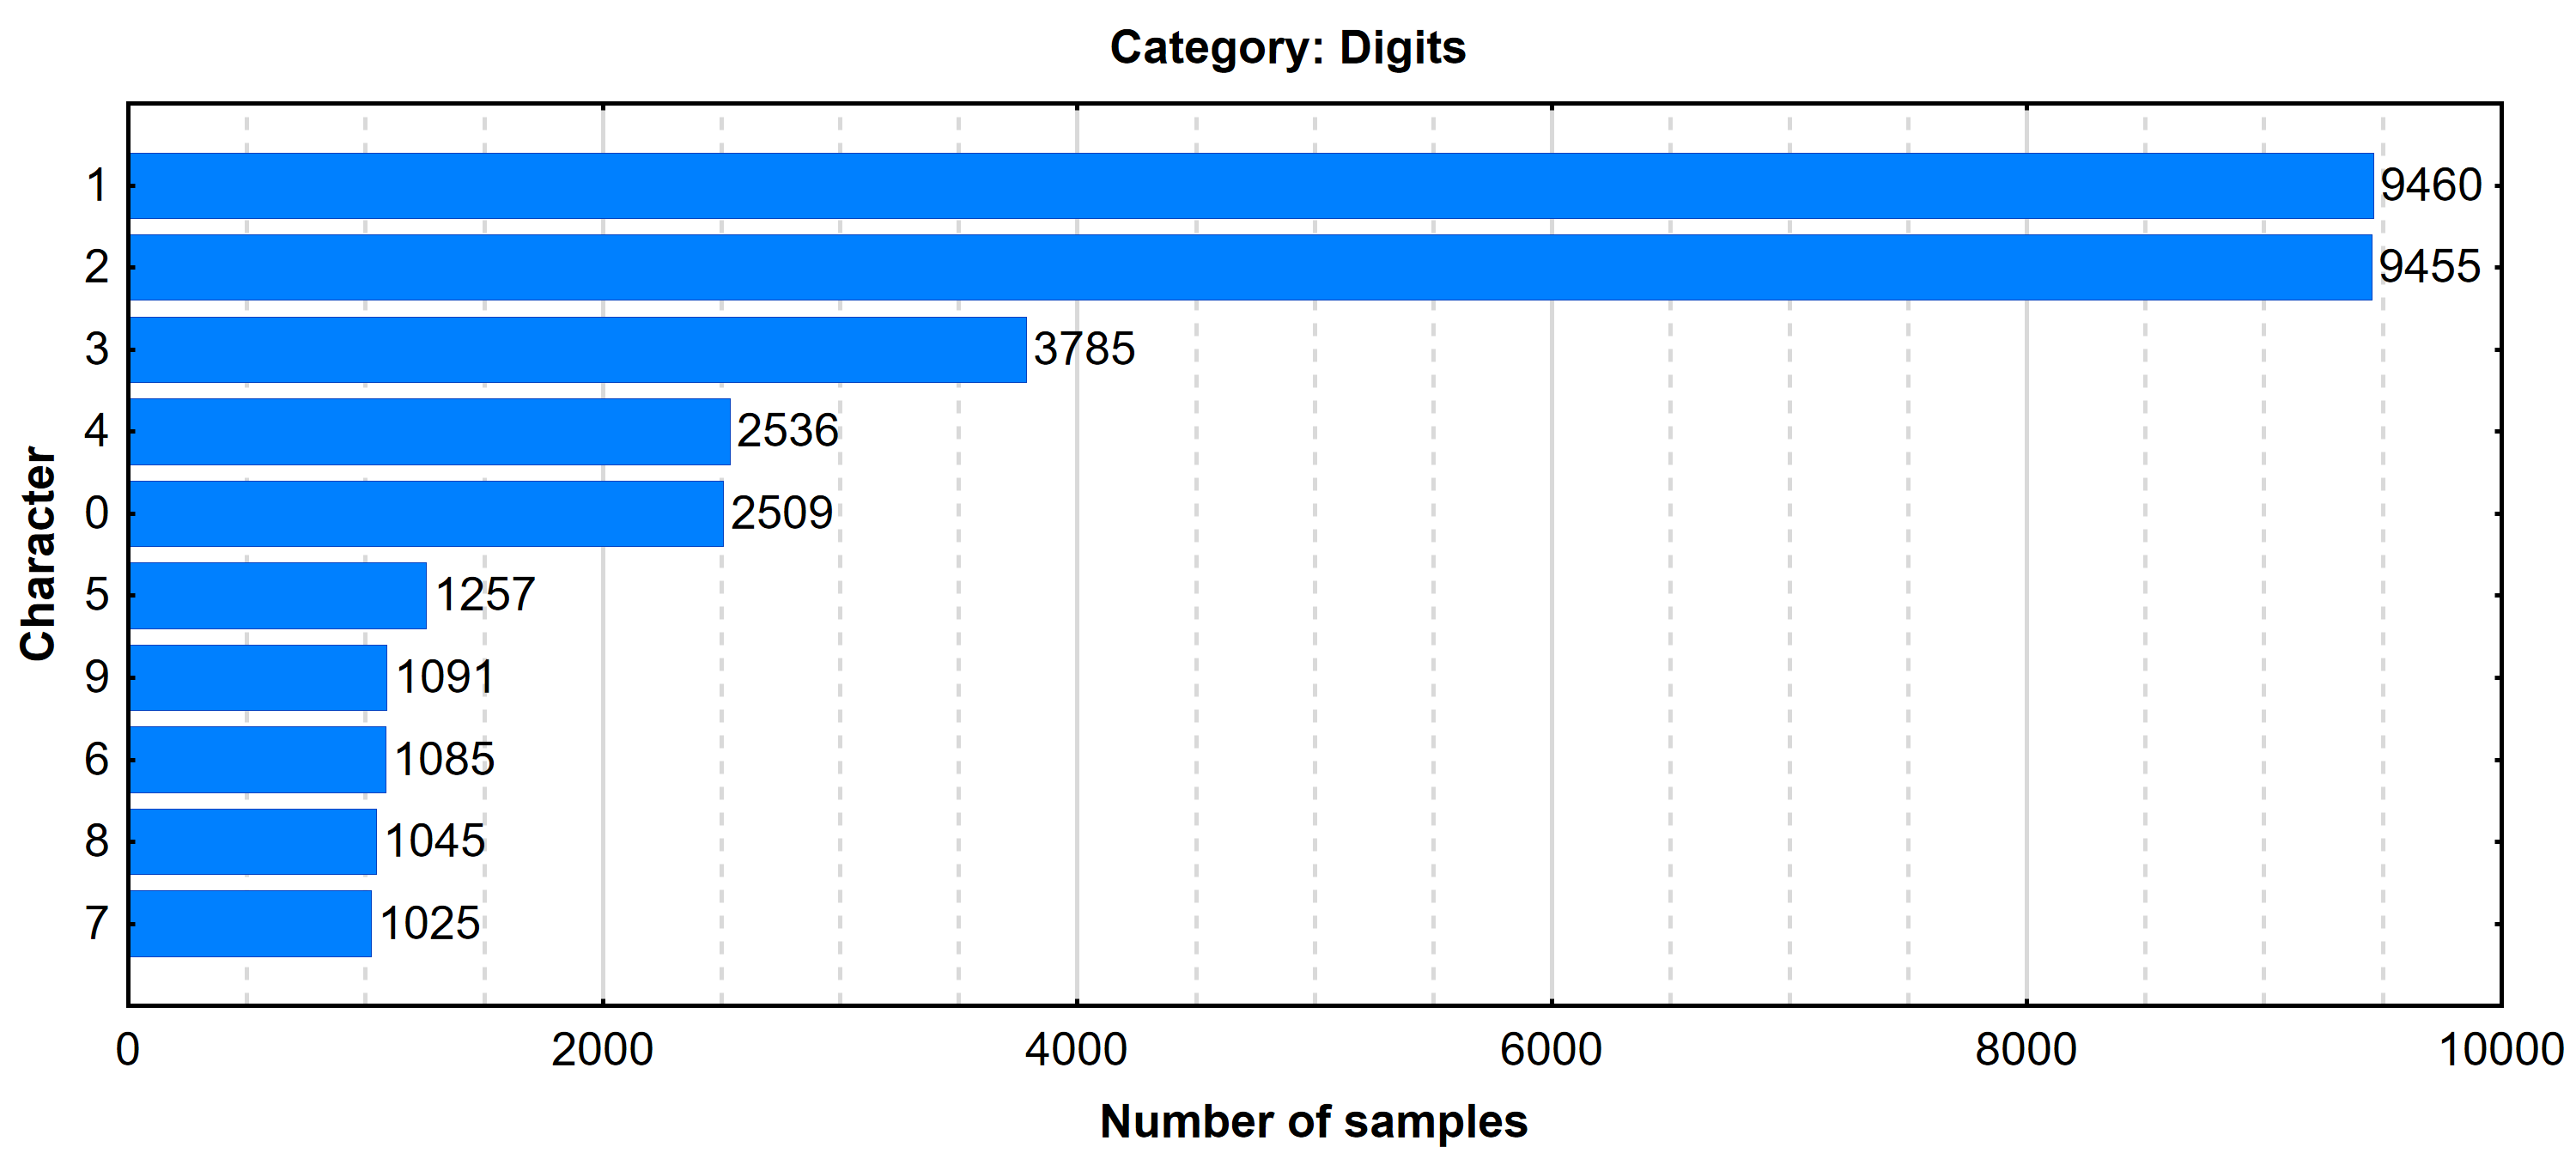
\includegraphics[width=1\textwidth]{capitulo3/imgs/digits_distribution.png}
	\caption{Frecuencia de aparición de dígitos del sistema de numeración arábigo \cite{EXTRACTOR}}
	\label{fig:DigDist}
\end{figure}
\newpage
En el caso de los símbolos matemáticos el de mayor aparición es el símbolo \textbf{-} con doce mil trecientas veintiocho veces. En esta gráfica podemos observar la aparición de símbolos que soportan expresiones que involucren divisiones o funciones trigonométricas o comparadores, incluso cuantificador de existencia aunque con una muy baja frecuencia de tan solo once apariciones.
\begin{figure}[H]
	\centering
	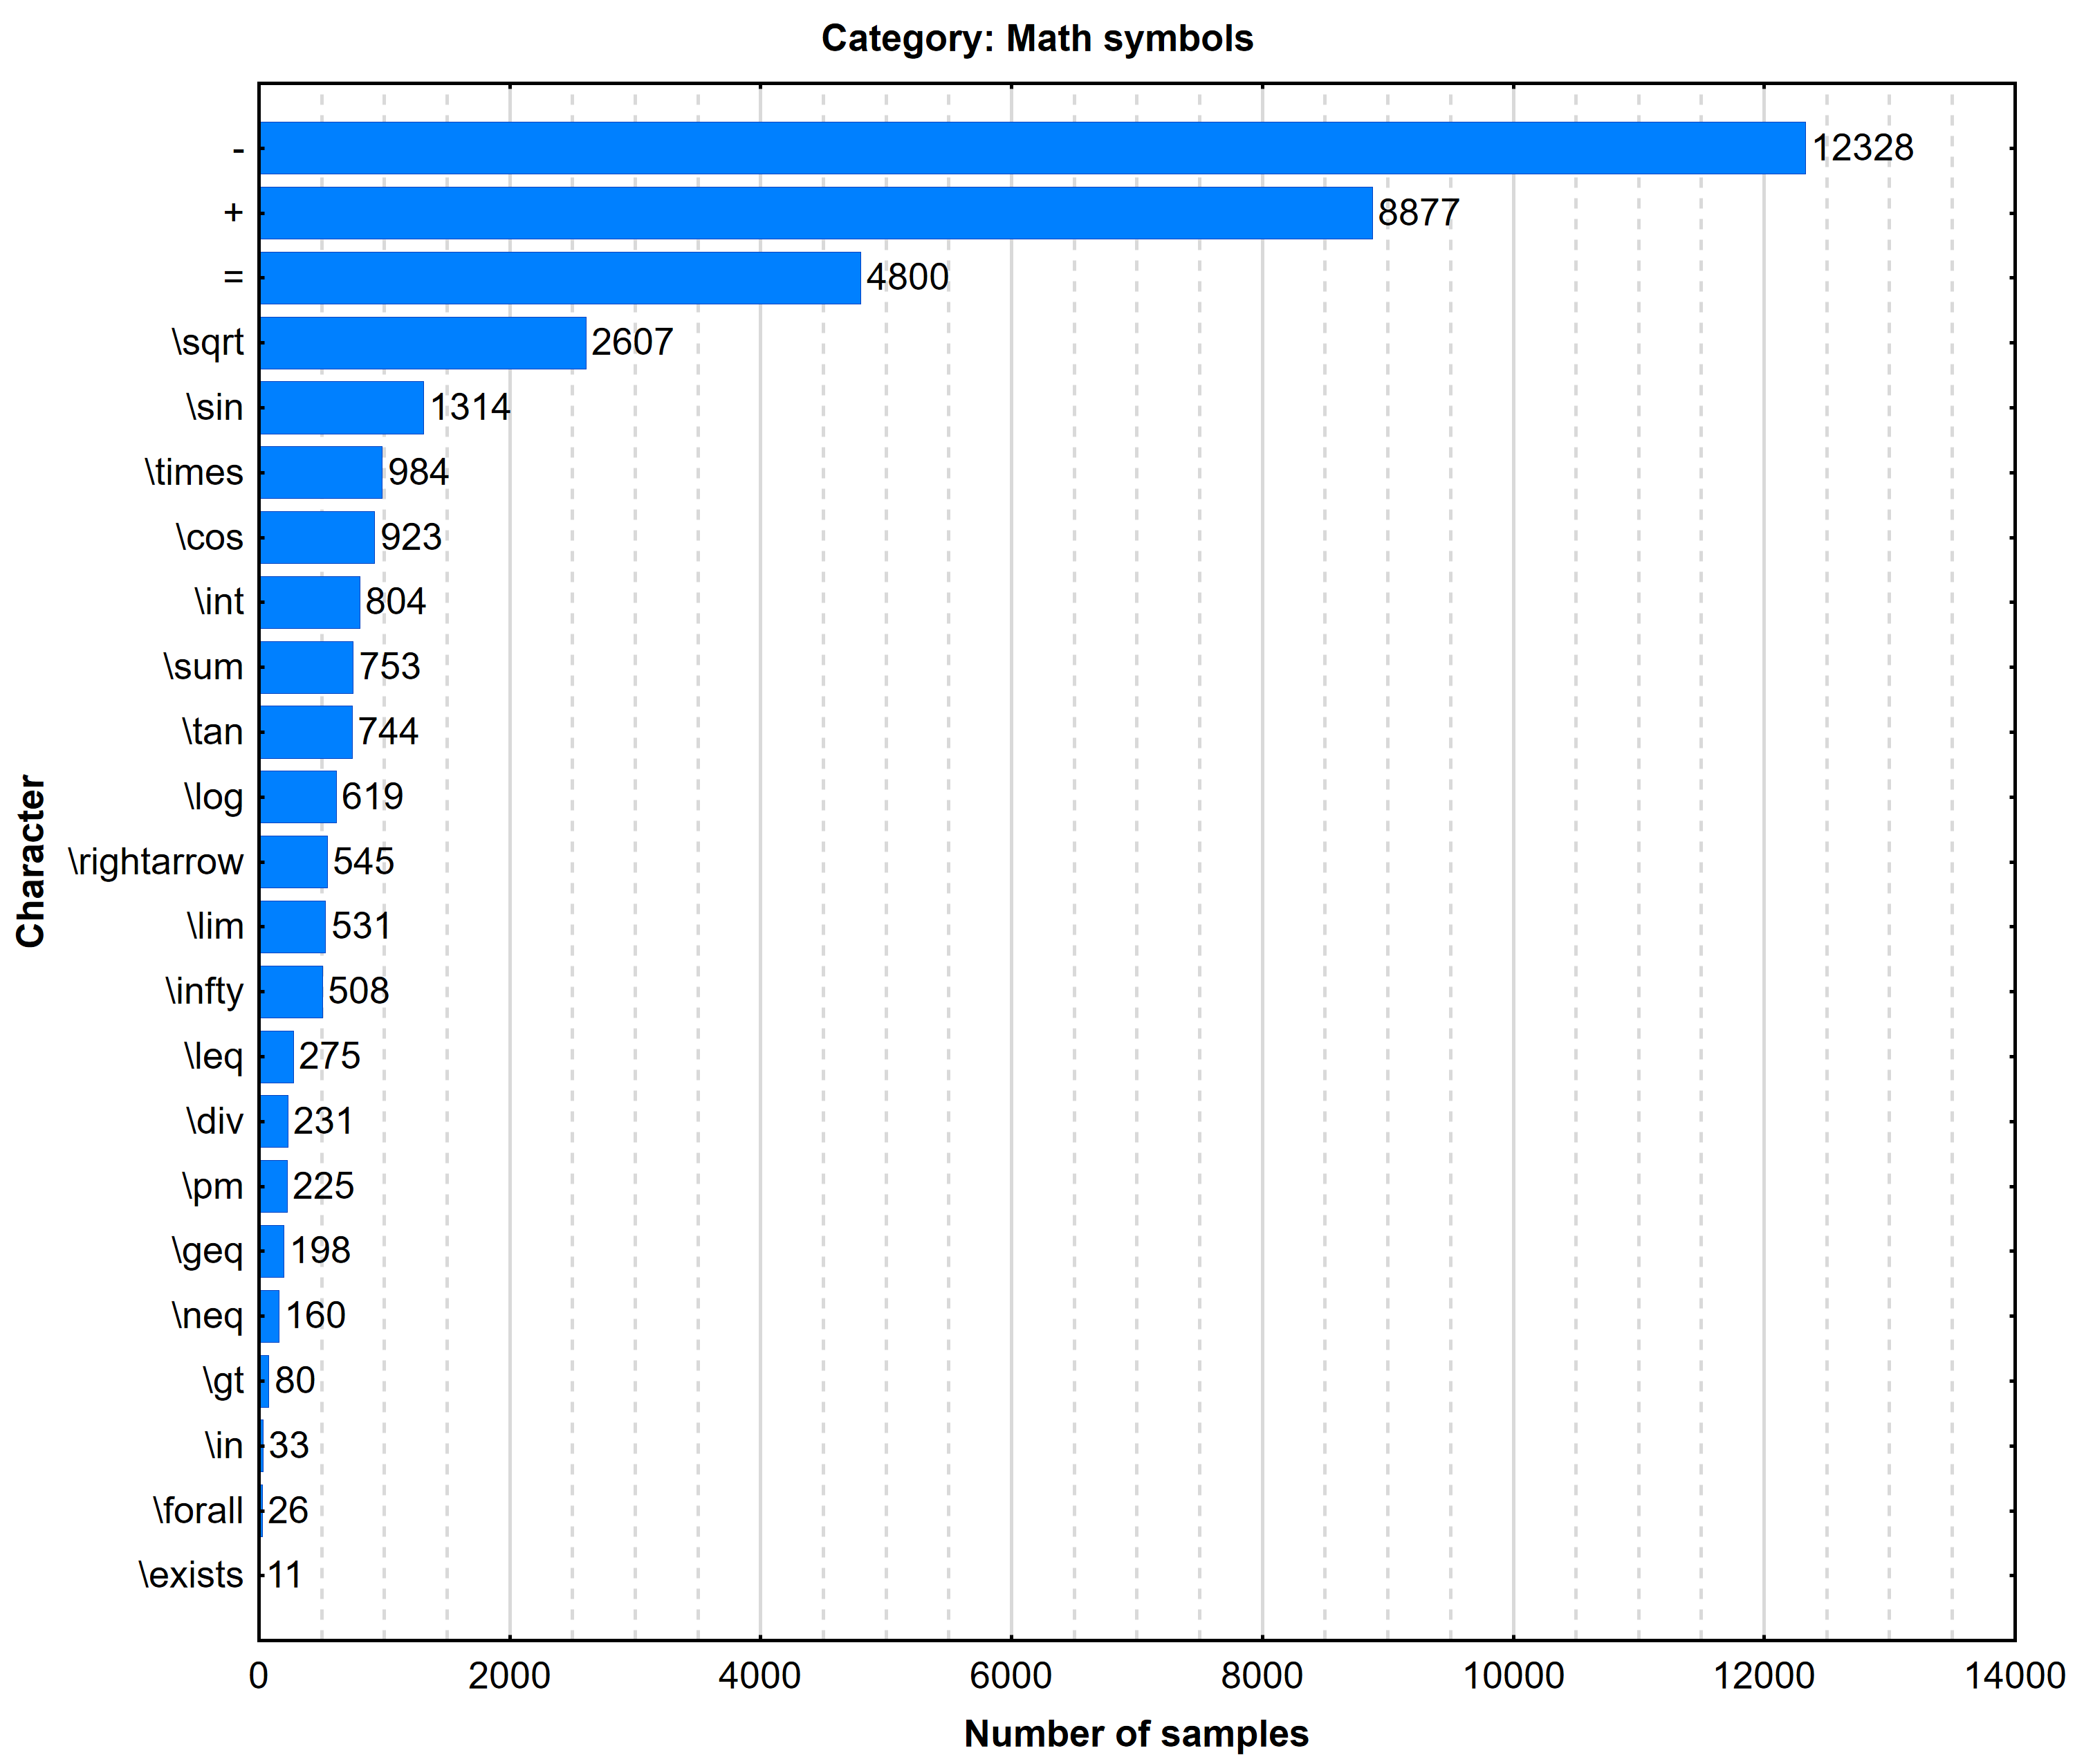
\includegraphics[width=1\textwidth]{capitulo3/imgs/math_symbols_distribution.png}
	\caption{Frecuencia de aparición de símbolos matemáticos \cite{EXTRACTOR}}
	\label{fig:MathSymbols}
\end{figure}
\newpage

En el caso de letras mayúsculas se logró identificar una frecuencia de cuatrocientos sesenta y nueve para el caso de la letra \textbf{C} mientras que para la letra \textbf{I} de noventa y seis.
\begin{figure}[H]
	\centering
	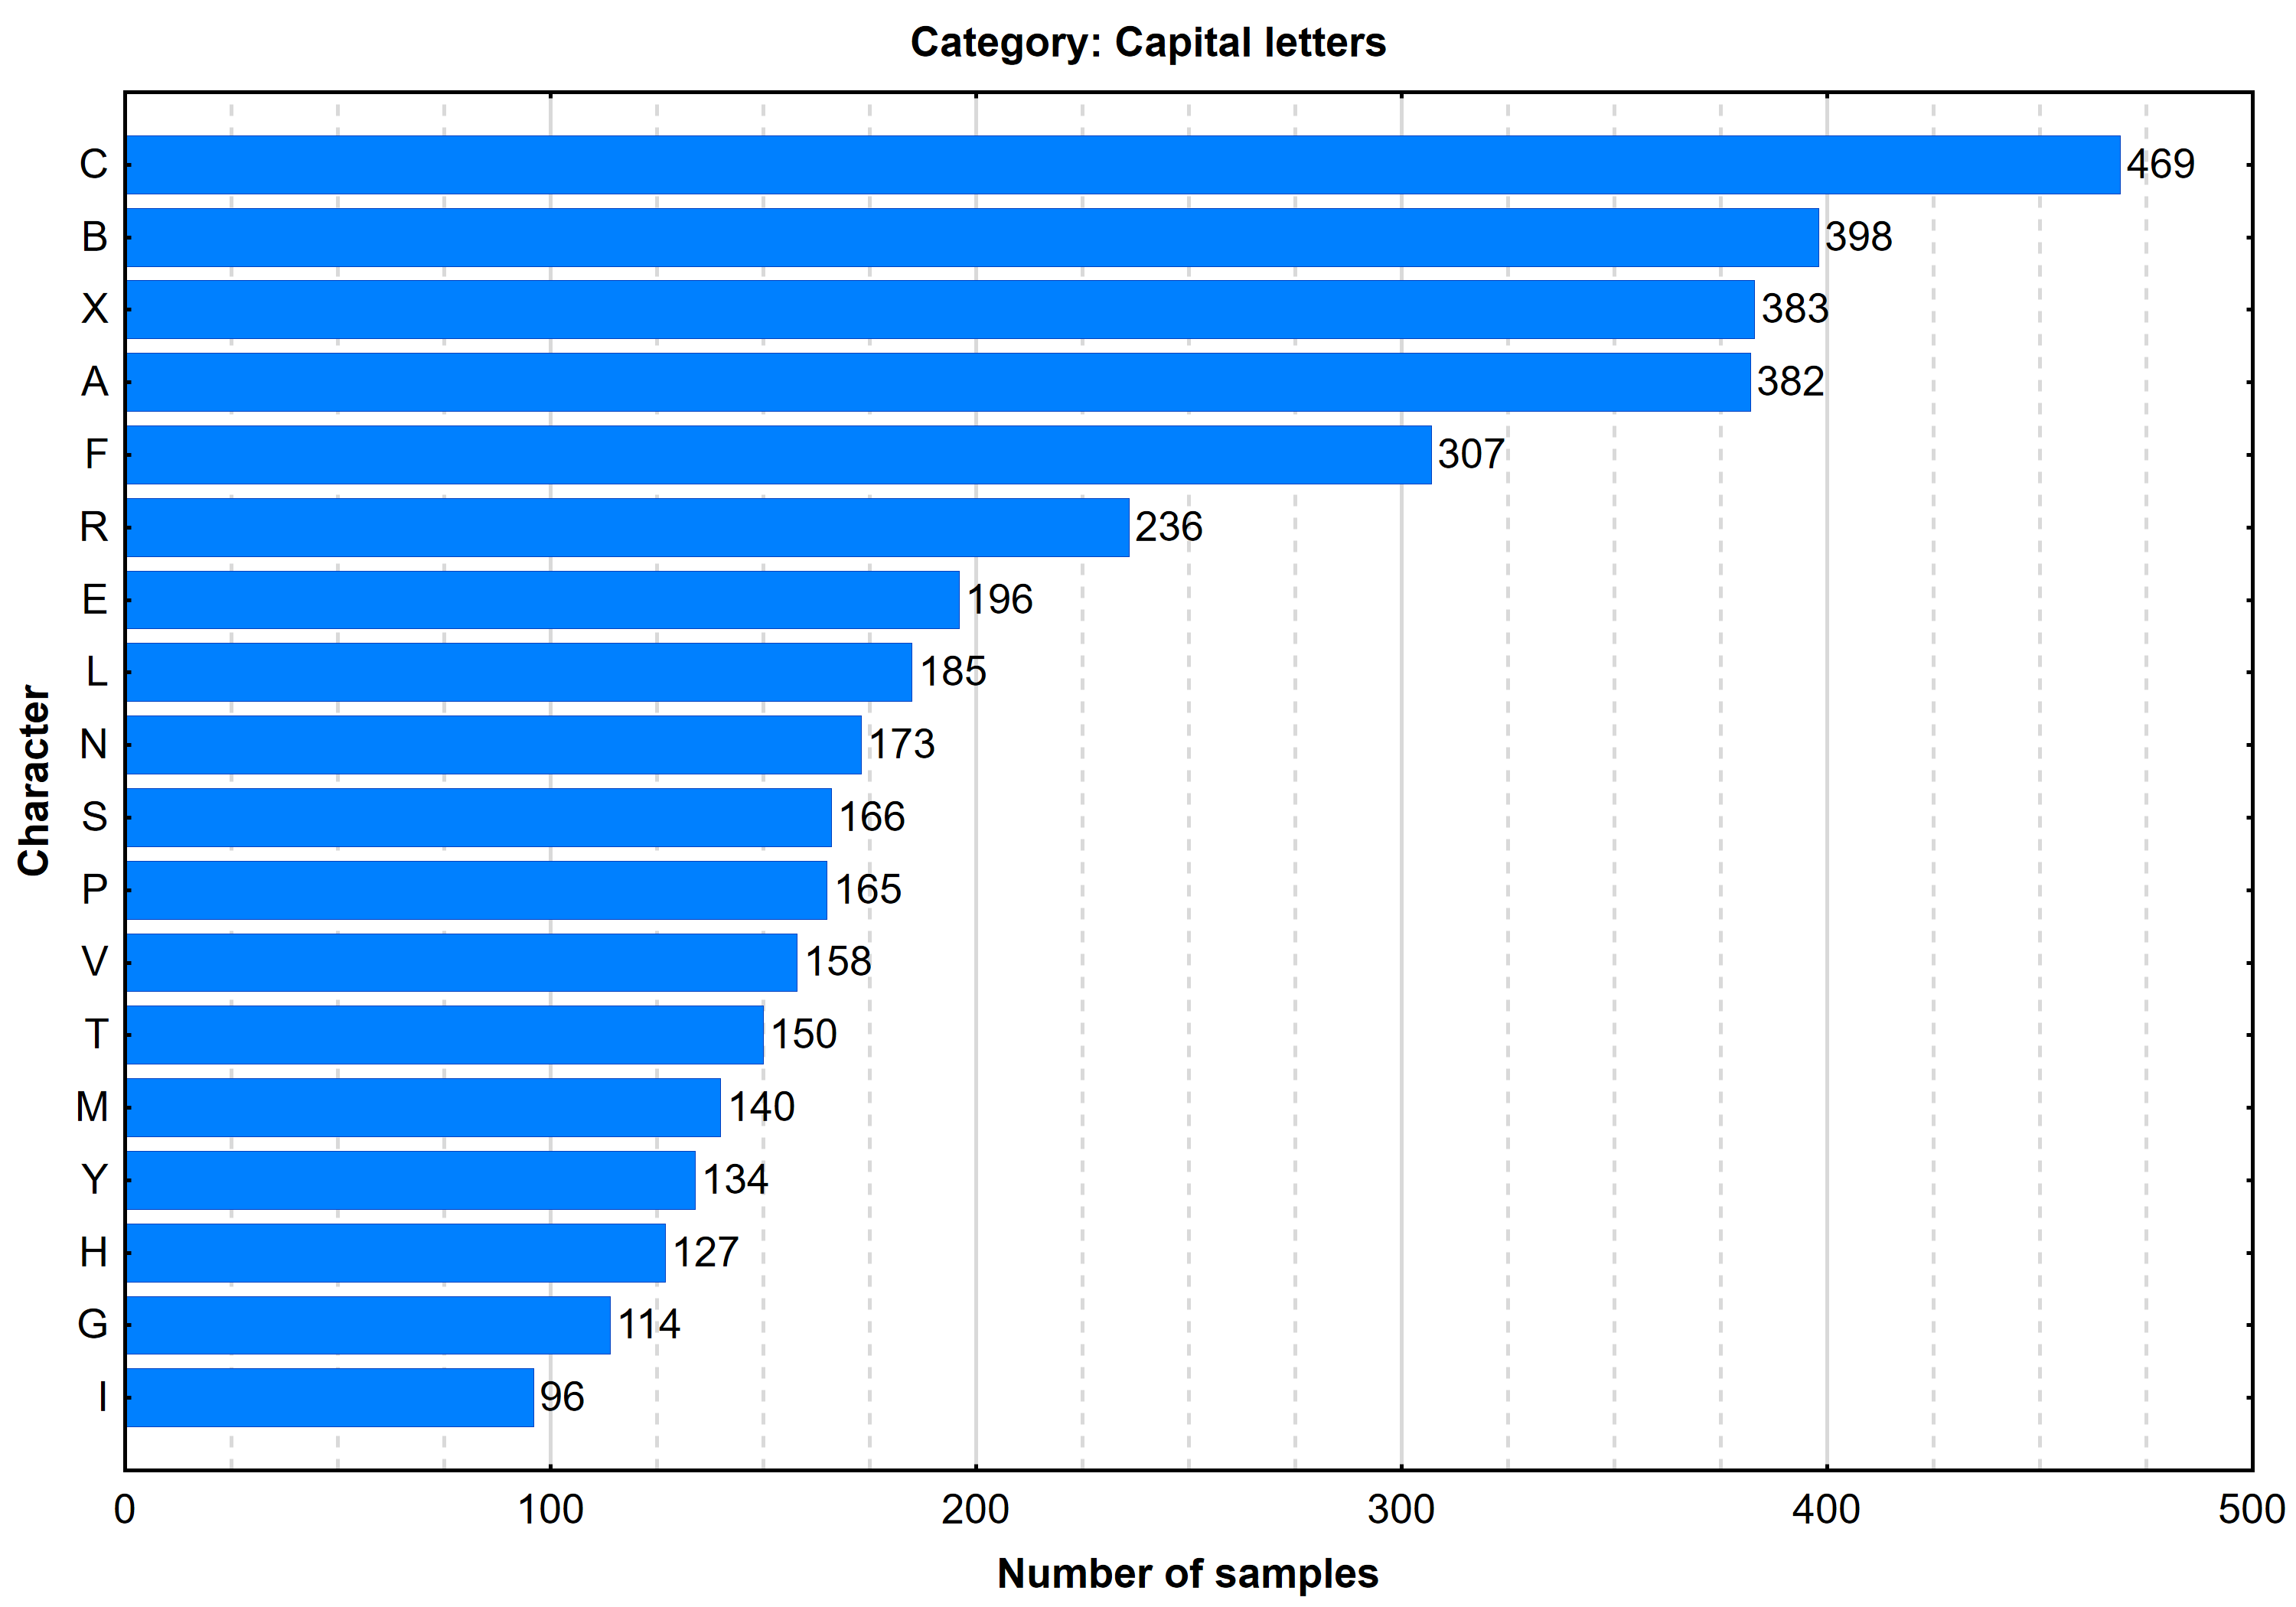
\includegraphics[width=1\textwidth]{capitulo3/imgs/capital_letters_distribution.png}
	\caption{Frecuencia de aparición de letras mayúsculas \cite{EXTRACTOR}}
	\label{fig:CapLetters}
\end{figure}
\newpage
En el caso de las letras minúsculas como podría esperarse la letra $\textbf{x}$ tiene la mayor aparición con ocho mil ciento nueve veces.
\begin{figure}[H]
	\centering
	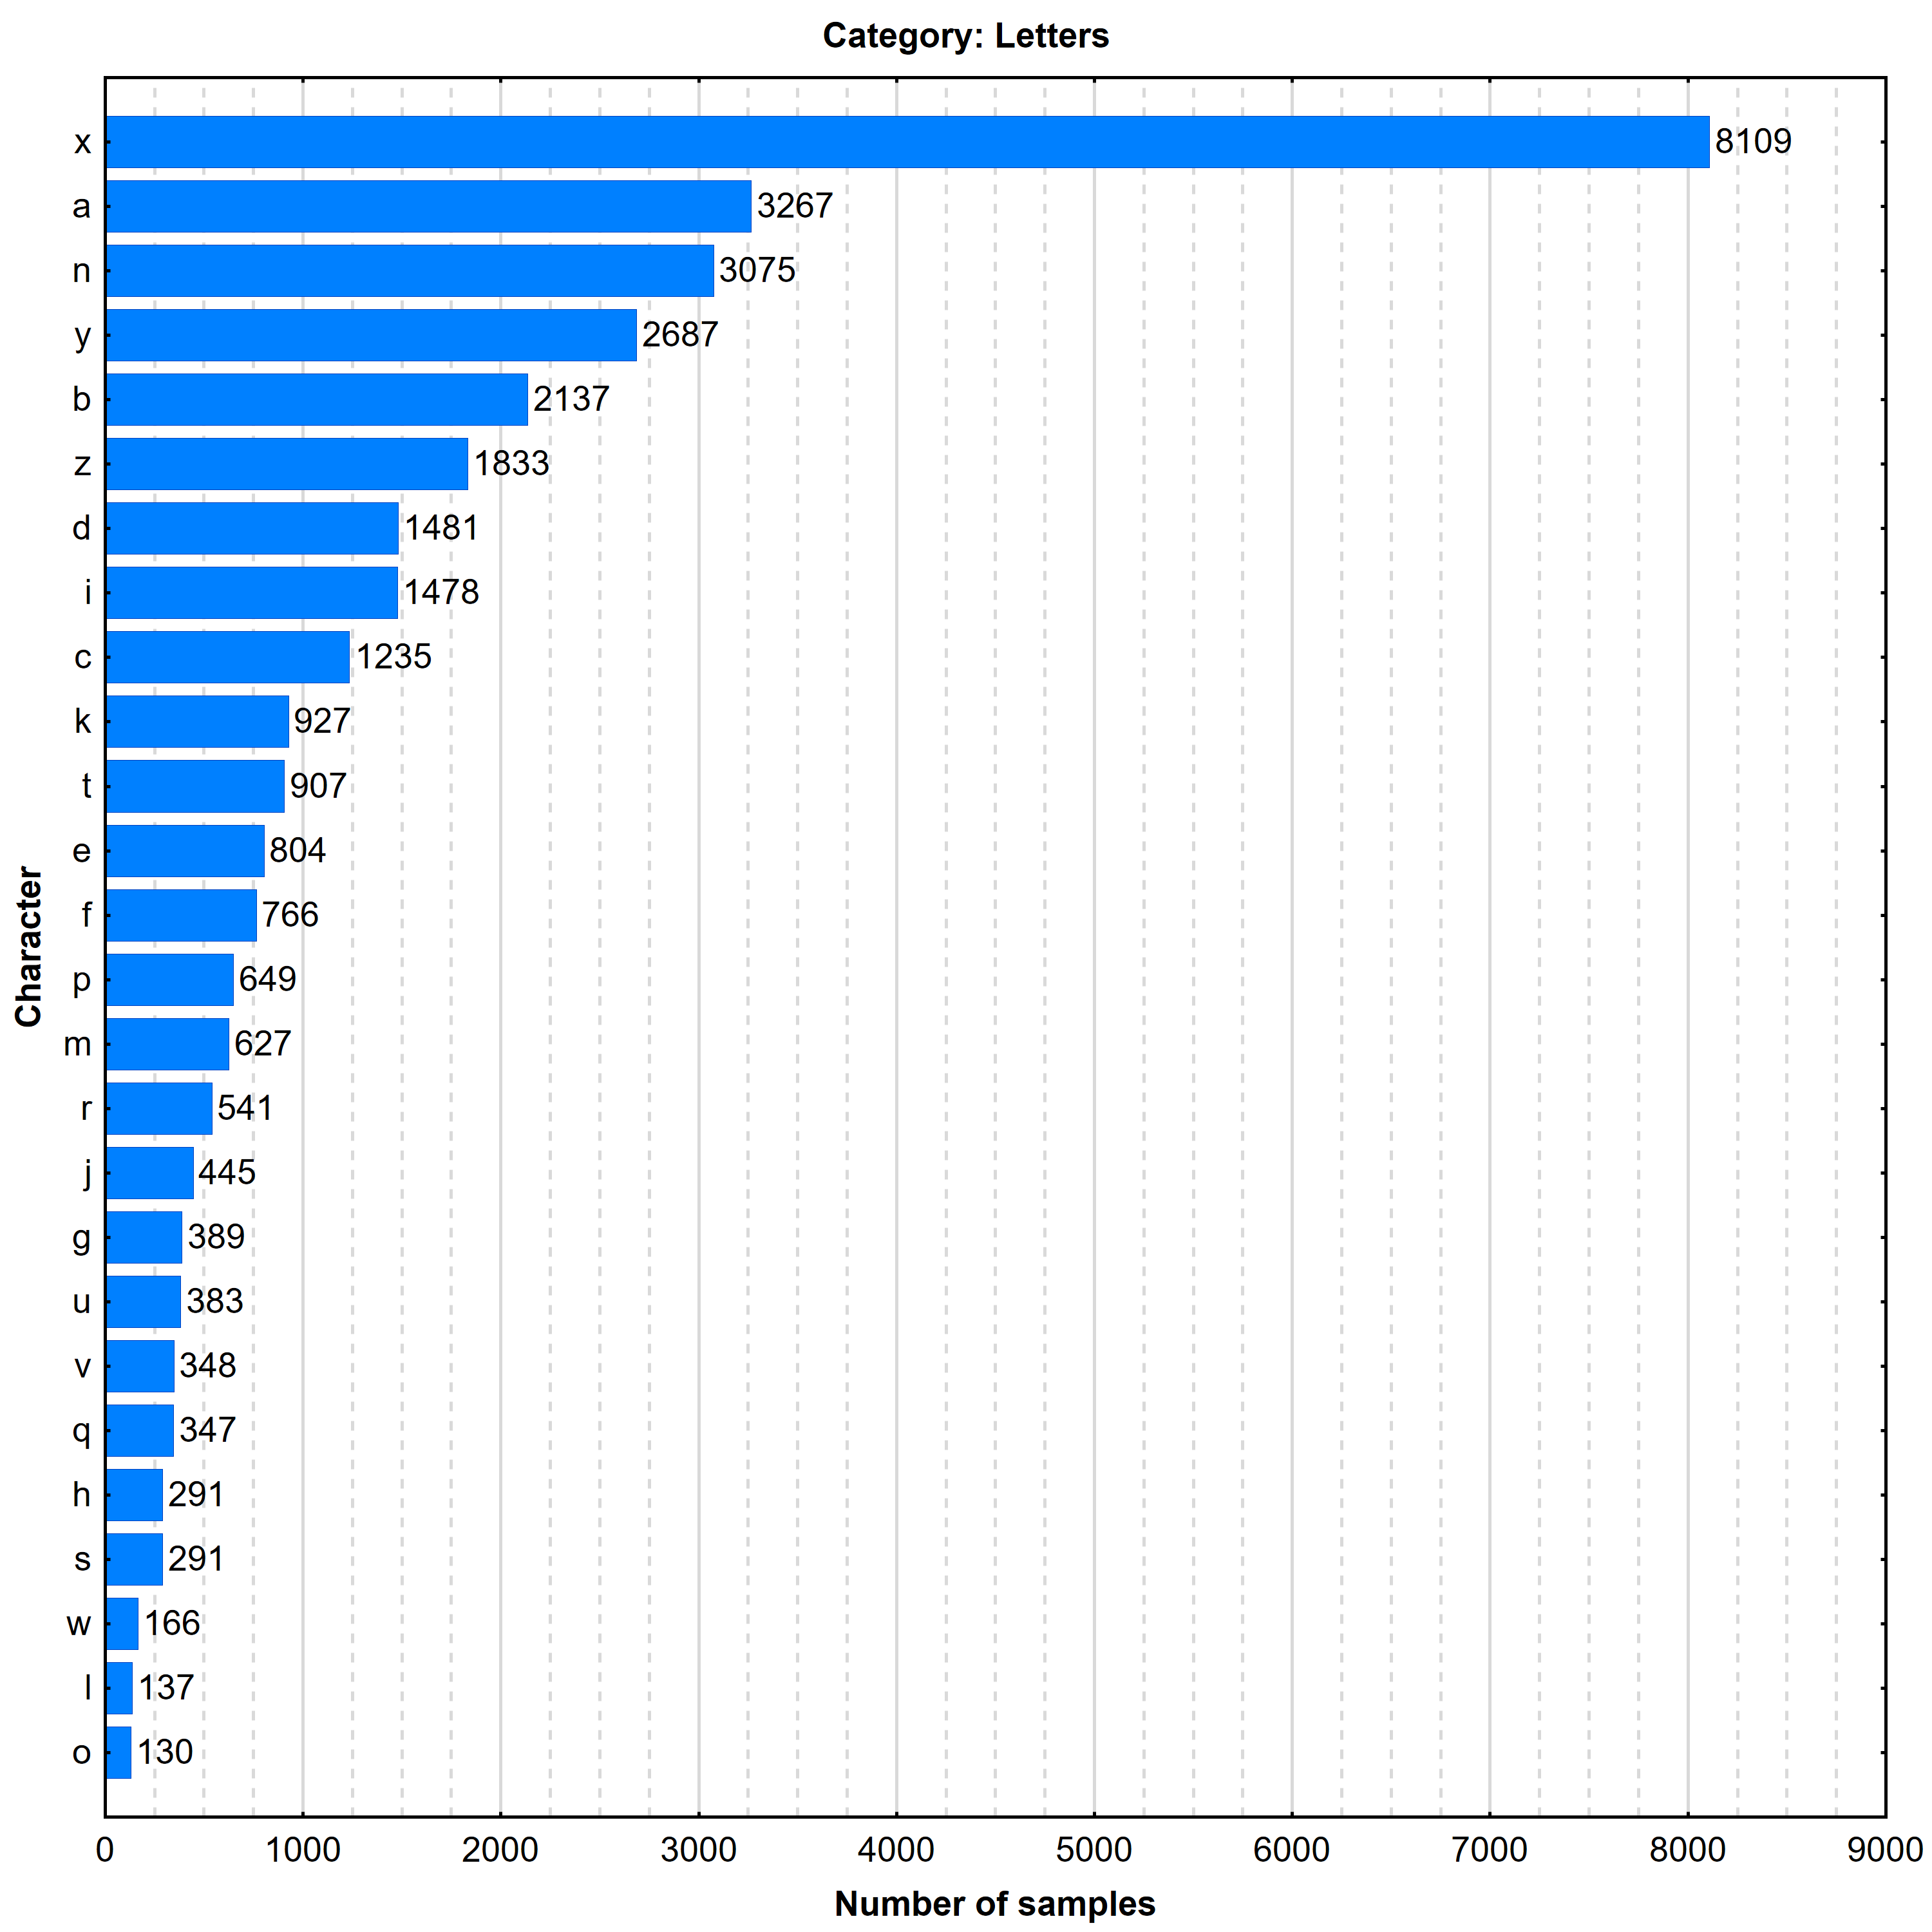
\includegraphics[width=1\textwidth]{capitulo3/imgs/lowercase_letters_distribution.png}
	\caption{Frecuencia de aparición de letras minúsculas \cite{EXTRACTOR}}
	\label{fig:LowerLetters}
\end{figure}
\newpage
La categoría con menos elementos pertenece a las letras griegas con nueve caracteres, siendo $\alpha$ (alpha) el de mayor aparición con ochocientas diecinueve veces.
\begin{figure}[H]
	\centering
	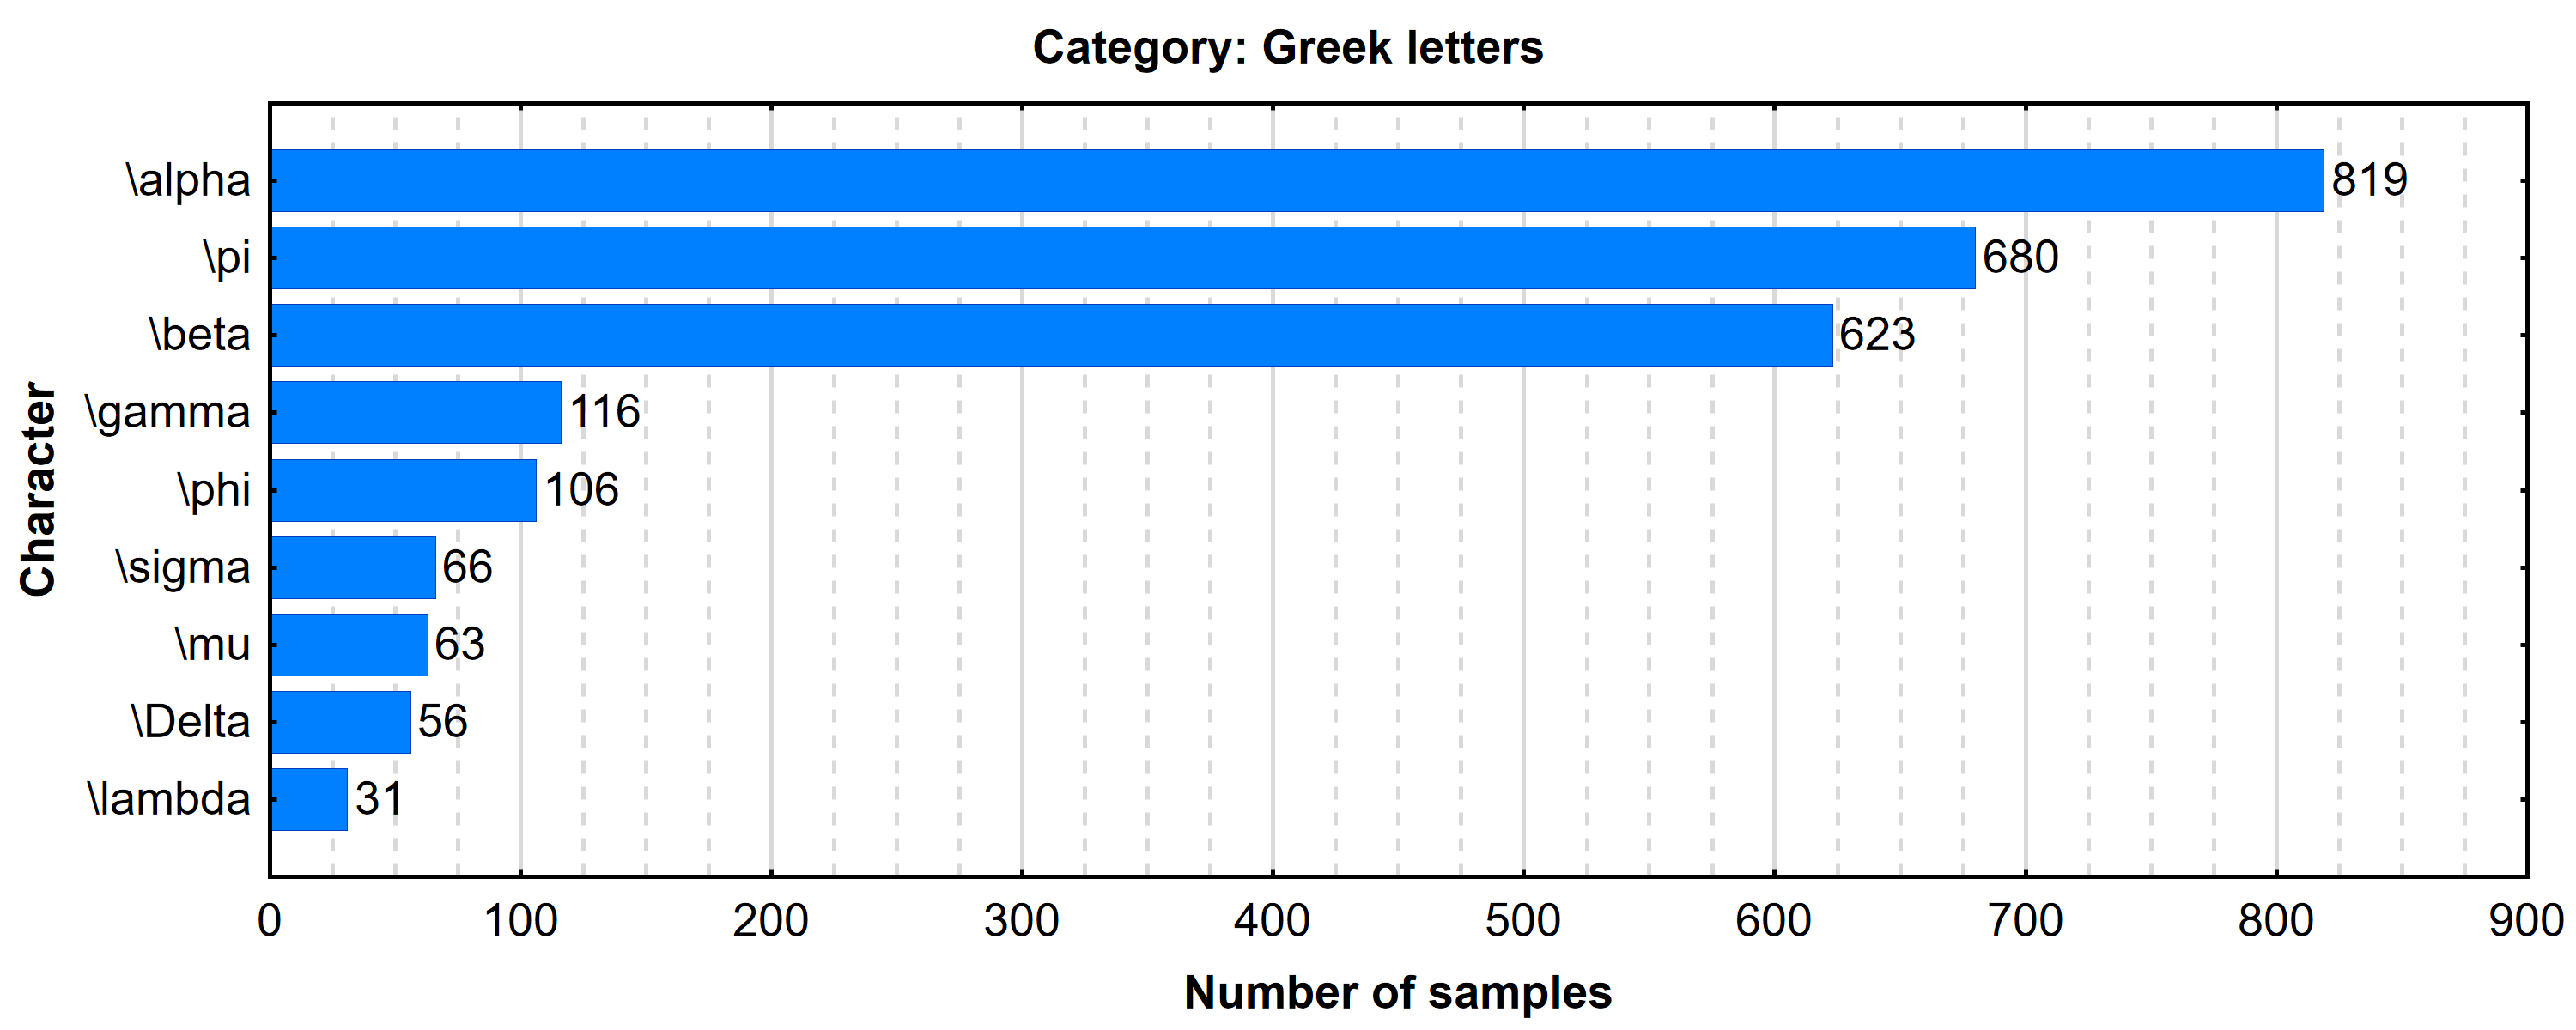
\includegraphics[width=1\textwidth]{capitulo3/imgs/greek_letters_distribution.png}
	\caption{Frecuencia de aparición de letras griegas \cite{EXTRACTOR}}
	\label{fig:GreekLetters}
\end{figure}
\newpage
Otros caracteres que aparecen en el conjunto de entrenamiento se muestran en la figura \ref{fig:SpecialSymbols} que son también de bastante utilidad como paréntesis, llaves, corchetes, el punto y la coma, que permiten definir jerarquía en las operaciones o números de punto flotante por mencionar dos aplicaciones que muestran la utilidad de los mismos. 
\begin{figure}[H]
	\centering
	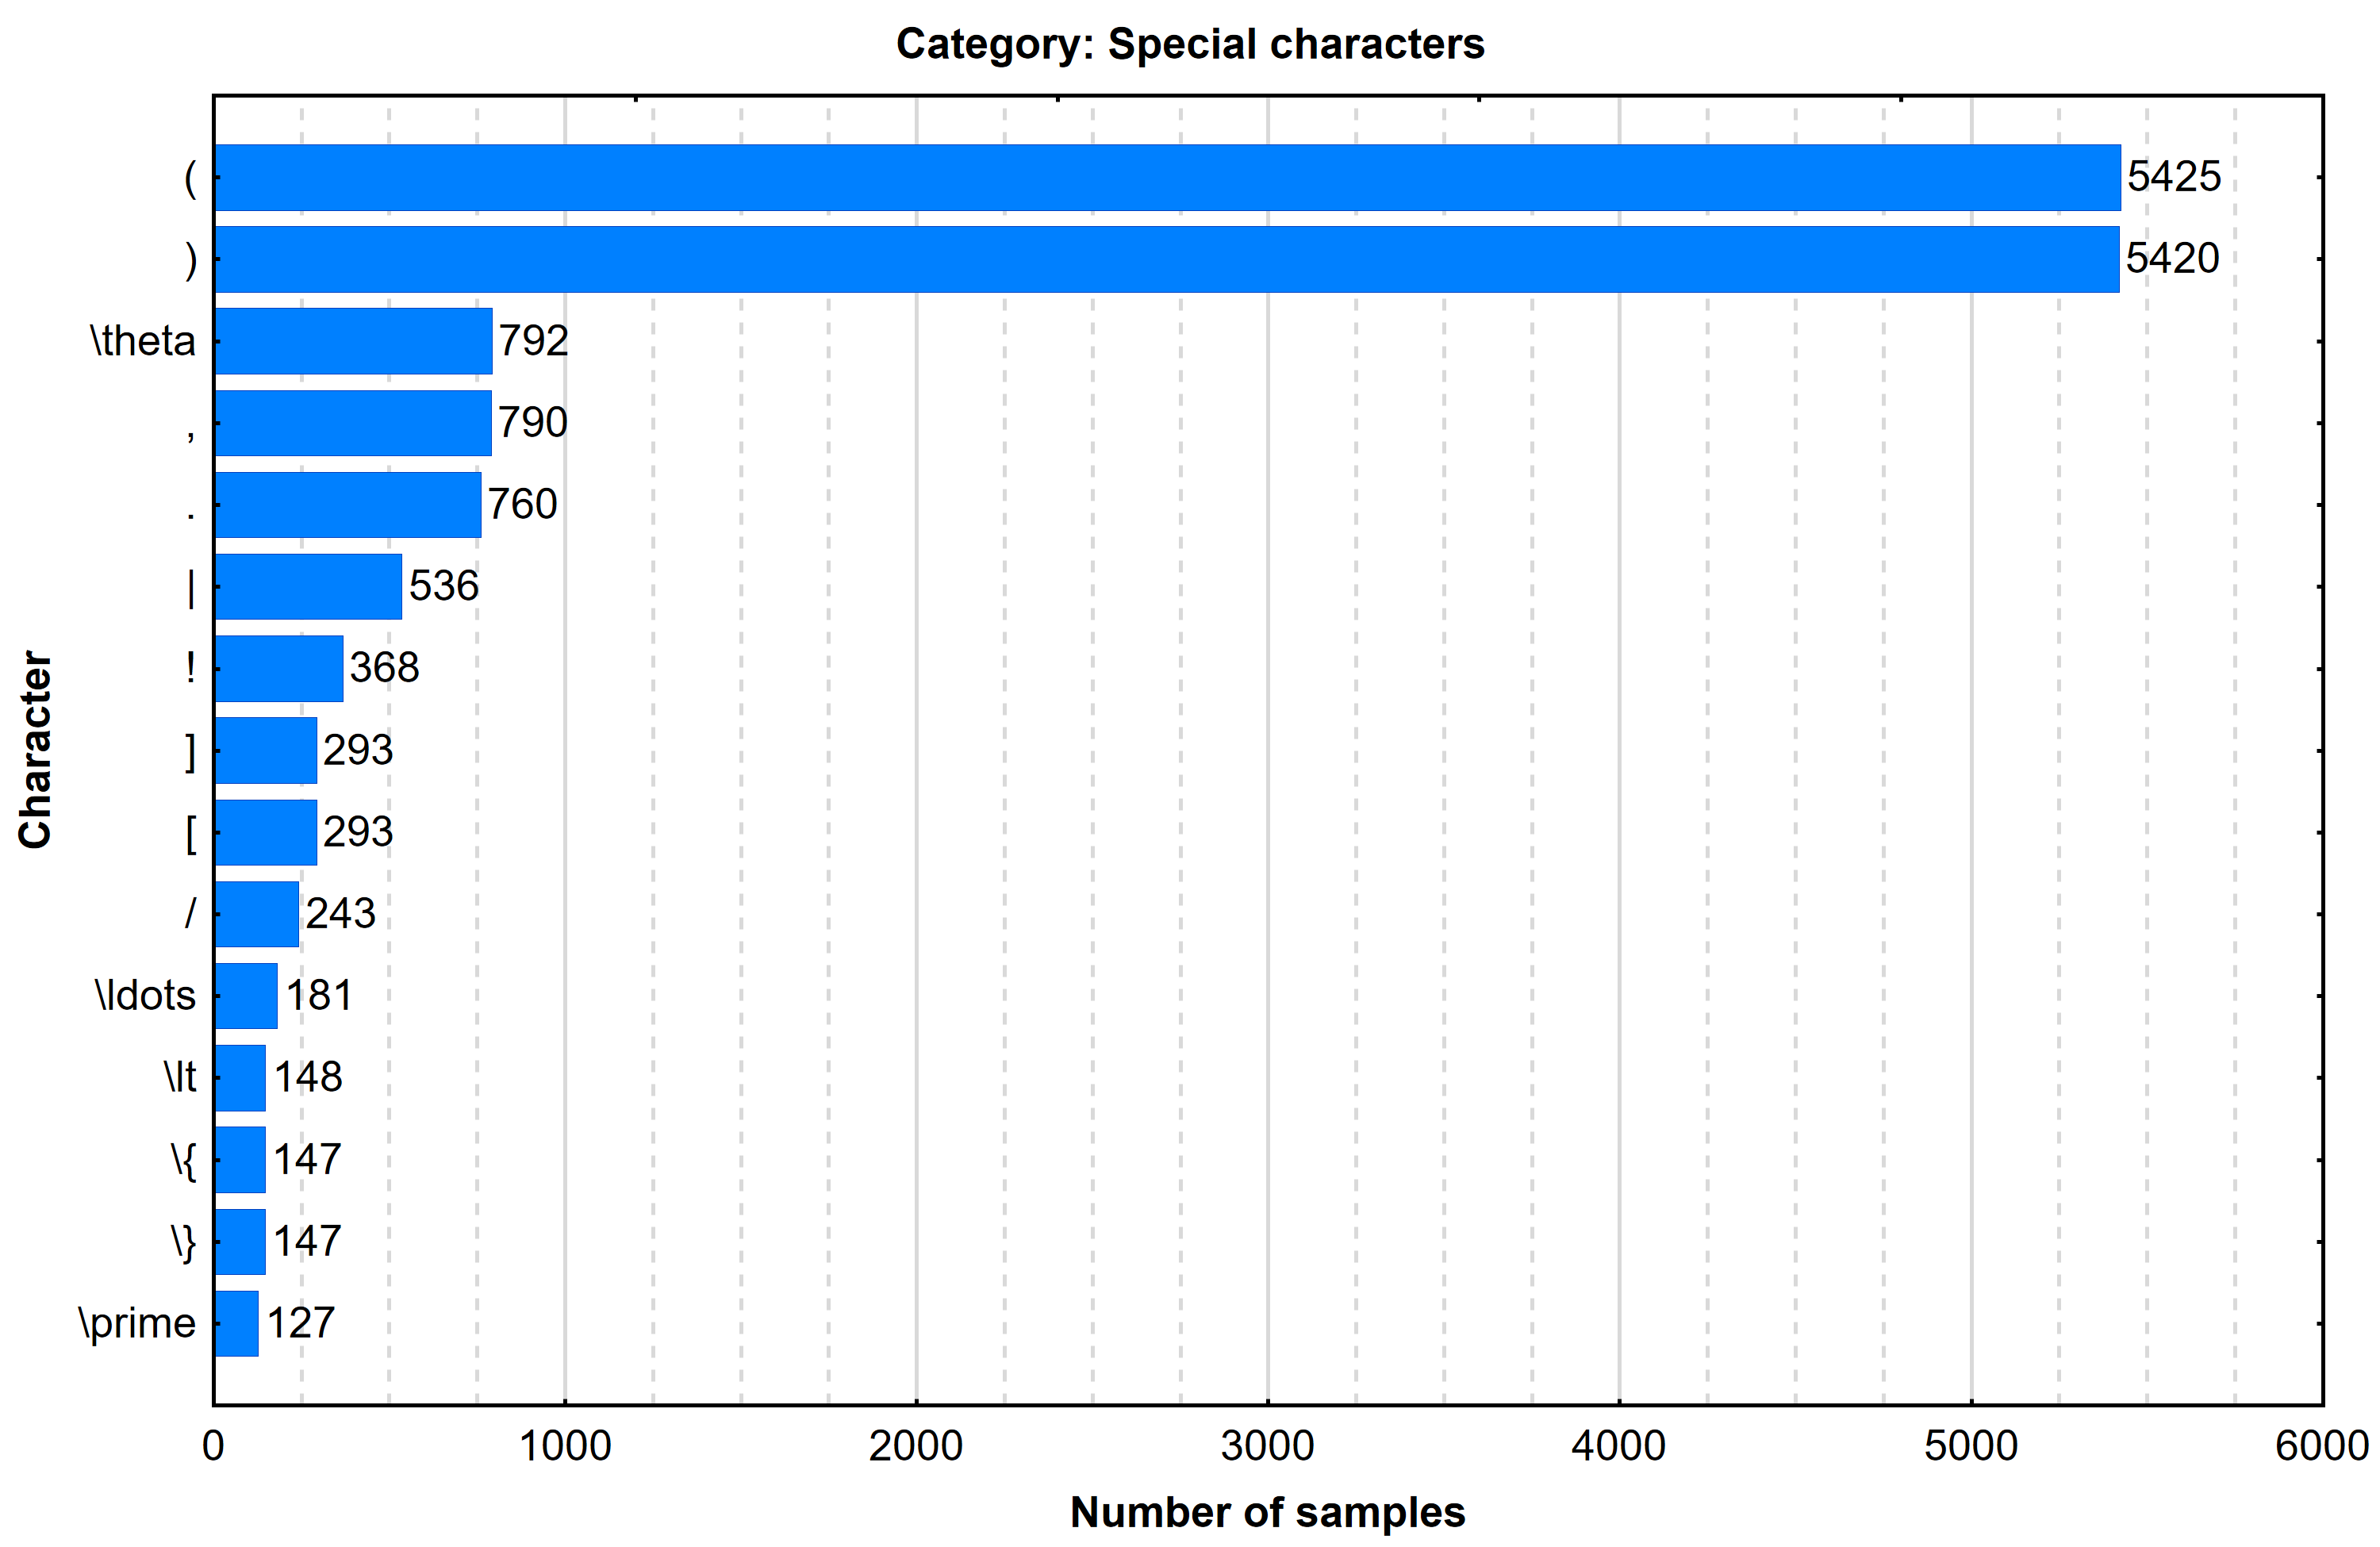
\includegraphics[width=1\textwidth]{capitulo3/imgs/special_characters_distribution.png}
	\caption{Frecuencia de aparición de símbolos especiales \cite{EXTRACTOR}}
	\label{fig:SpecialSymbols}
\end{figure}

Con estos histogramas se puede determinar qué símbolos se espera puedan ser reconocidos, así como aquellos de los cuales se esperan mejores resultados en función de su frecuencia de aparición en el conjunto de entrenamiento.

\newpage
\subsection{Nivel dimensional}
Sabiendo que el conjunto de entrenamiento CROHME no es lo suficientemente grande siendo esta una de las limitantes para obtener buenos resultados y teniendo en cuenta la bidimensionalidad que se presenta en las expresiones matemáticas, se propone el reconocimiento dos niveles en ambas direcciones, teniendo esta restricción con un mayor peso en dirección perpendicular al sentido de la escritura de las expresiones, esto basado en los resultados obtenidos por \cite{chino} 
con el mismo conjunto de entrenamiento. La figura \ref{fig:TwoDimensions} muestra un ejemplo del conjunto de entrenamiento CROHME.
%insertar Imagen
\begin{figure}[H]
	\centering
	
\includegraphics[width=0.6\textwidth]{capitulo3/imgs/twolevel.jpeg}
	\caption{Expresión de dos niveles vertical}
	\label{fig:TwoDimensions}
\end{figure}
\section{Traducción de imágenes a \LaTeX}

El problema de traducir imágenes a \LaTeX automáticamente, es aún un campo de investigación abierto. Dada su naturaleza recursiva miltinivel, las inmensas ambigüedades en la escritura y su fuerte dependencia a un contexto claro, esta tarea difiere en gran medida del reconocimiento óptico de caracteres (OCR) para el cual ya existen sistemas con una precisión suficiente. \\

Según \cite{chino}, el reconocimiento de expresiones matemáticas a mano (HMER) comprende dos grandes problemas: reconocimiento de los símbolos y el análisis de su estructura. Existen dos grandes aproximaciones, las cuales son: secuenciales y globales. \\

Las aproximaciones secuenciales, buscan primero reconocer los símbolos y después realizán el análisis estructural por separado. Uno de los problemas que esta aproximación presenta, es que los errores cometidos en la parte del reconocimiento, serán heredados por el análisis estructural, generando una cadena de malas traducciones. La solución secuencial que mejores resultados ha dado, es el uso de grámaticas predefinidas para llevar a cabo el reconocimiento de la estructura de la expresión. \\

La segunda alternativa, combina los dos tipos de análisis en uno solo, pues busca ir reconociendo la estructura a la vez que se reconocen los símbolos. Esta aproximación permite generar la segmentación de símbolos utilizando toda la información disponible de la imagen, por lo que este tipo de soluciones parecen ser una mejor opción, sin embargo, este procedimiento es más costoso computacionalmente. Recientes investigaciones, han utilizado las arquitecturas encoder-decoder mencionadas previamente en el Marco Teórico para atacar el problema de forma global como si fuera una tarea de Image Captioning. Los resultados obtenidos por este tipo de aproximación resultan ser menos costos y más precisos. \\

Las dos propuestas principales, es decir, las gramáticas y la arquitectura encoder-decoder tienen sus limitaciones. En el caso de las gramáticas, podemos ver que los algoritmos para el procesamiento de las mismas incrementan su complejidad exponencialmente entre más expresiones son capaces de reconocer, además de que requieren un conocimiento previo de los símbolos. Mientras que con el avance de los procesadores y GPUs las aproximaciones globales con redes neuronales se vuelven cada vez más plausibles y es por esta razón que los investigadores en el campo del machine learning le han prestado particular atención mejorando así, los resultados obtenidos por cualquier otro método. \\

En el presente Trabajo Terminal, se ha decidido utilizar la aproximación global propuesta por \cite{chino}, la cual es llamada Watch, Attend, Parse (WAP) que es una RNN encoder-decoder con un sistema de atención que permite reconocer expresiones matemáticas escritas a mano con una precisión del 46.55\%. En la Figura \ref{fig:wap} podemos ver un diagrama de esta arquitectura.\\

\begin{figure}[H]
	\centering
	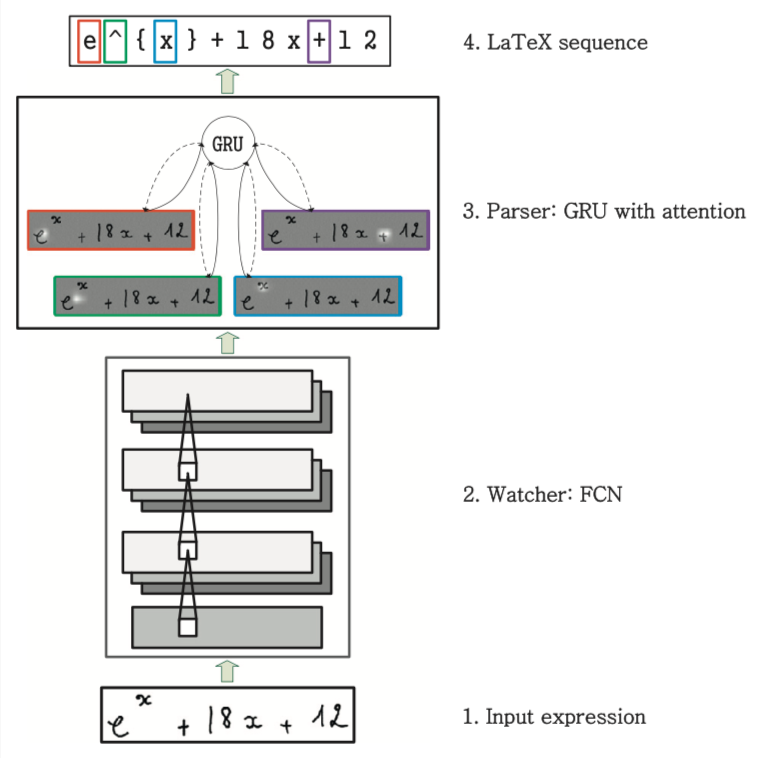
\includegraphics[]{capitulo3/imgs/wap}
	\caption{Diagrama de la arquitectura Watch, Attend, Parse (WAP).}
	\label{fig:wap}
\end{figure}

La red WAP, se compone de dos partes:

\begin{enumerate}
	\item \textbf{Encoder}: El cual es una CNN que permite extraer las características de la imagen y sumarizarlas en un vector de contexto $C$.
	\item  \textbf{Decoder}: El cual es una LSTM que toma el contexto $C$ y junto con sistema de atención retorna como salida la secuencia de símbolos de \LaTeX, un símbolo a la vez.
\end{enumerate}

